\vfill\null\columnbreak
\section{Design von Regelungssystemen}
    \subsection{Frequenzbedingung des geschlossenen Regelkreises}
        \subsubsection{Frequenzeigenschaften von Störungen und Rauschen}
            Die Übertragungsfunktionen des geschlossenen Regelkreises $S(s)$ und $T(s)$ sind intrinsisch gekoppelt:
            \[T(s) + S(s) = \frac{L(s)}{1+L(s)}+\frac{1}{1+L(s)}=1,\forall s\in\mathbb{C}\]
            Dies setzt voraus, dass bei gegebener Frequenz $\overset{*}{\omega}$ entweder $|T(j\overset{*}{\omega}|$ oder $|S(j\overset{*}{\omega})|$ viel kleiner als 1 sein kann.
            \textbf{Störungen} werden mit $S(s)$ auf den Ausgang übertragen und \textbf{Rauschen} mit $T(s)$.
            Die generelle Aufgabe eines Reglers ist die gleichzeitige Unterdrückung von Rauschen und Störungen. Dies ist jedoch nur möglich wenn die Signale in unterschiedlichen Frequenzbändern auftreten. Dabei tritt Rauschen in der Regel bei hohen Frequenzen $(\omega>\omega_n)$ auf und Störungen in der Regel bei tiefen Frequenzen $(\omega<\omega_d)$. Daraus ergibt sich folgende Erkenntnis:
        
            \textbf{Niedrige Frequenzen} $\boldsymbol{\omega<\omega_d}$
            \[|S(j\omega)| = \bigg|\frac{1}{1+L(j\omega)}\bigg|  \overset{!}{<<} 1 \Rightarrow 
            |L(j\omega)| >> 1 \]
            \textbf{Hohe Frequenzen} $\boldsymbol{\omega > \omega_n}$
            \[|T(j\omega)| = \bigg|\frac{L(j\omega)}{1+L(j\omega)}\bigg|  \overset{!}{<<} 1 \Rightarrow 
            |L(j\omega)| << 1 \]
       
            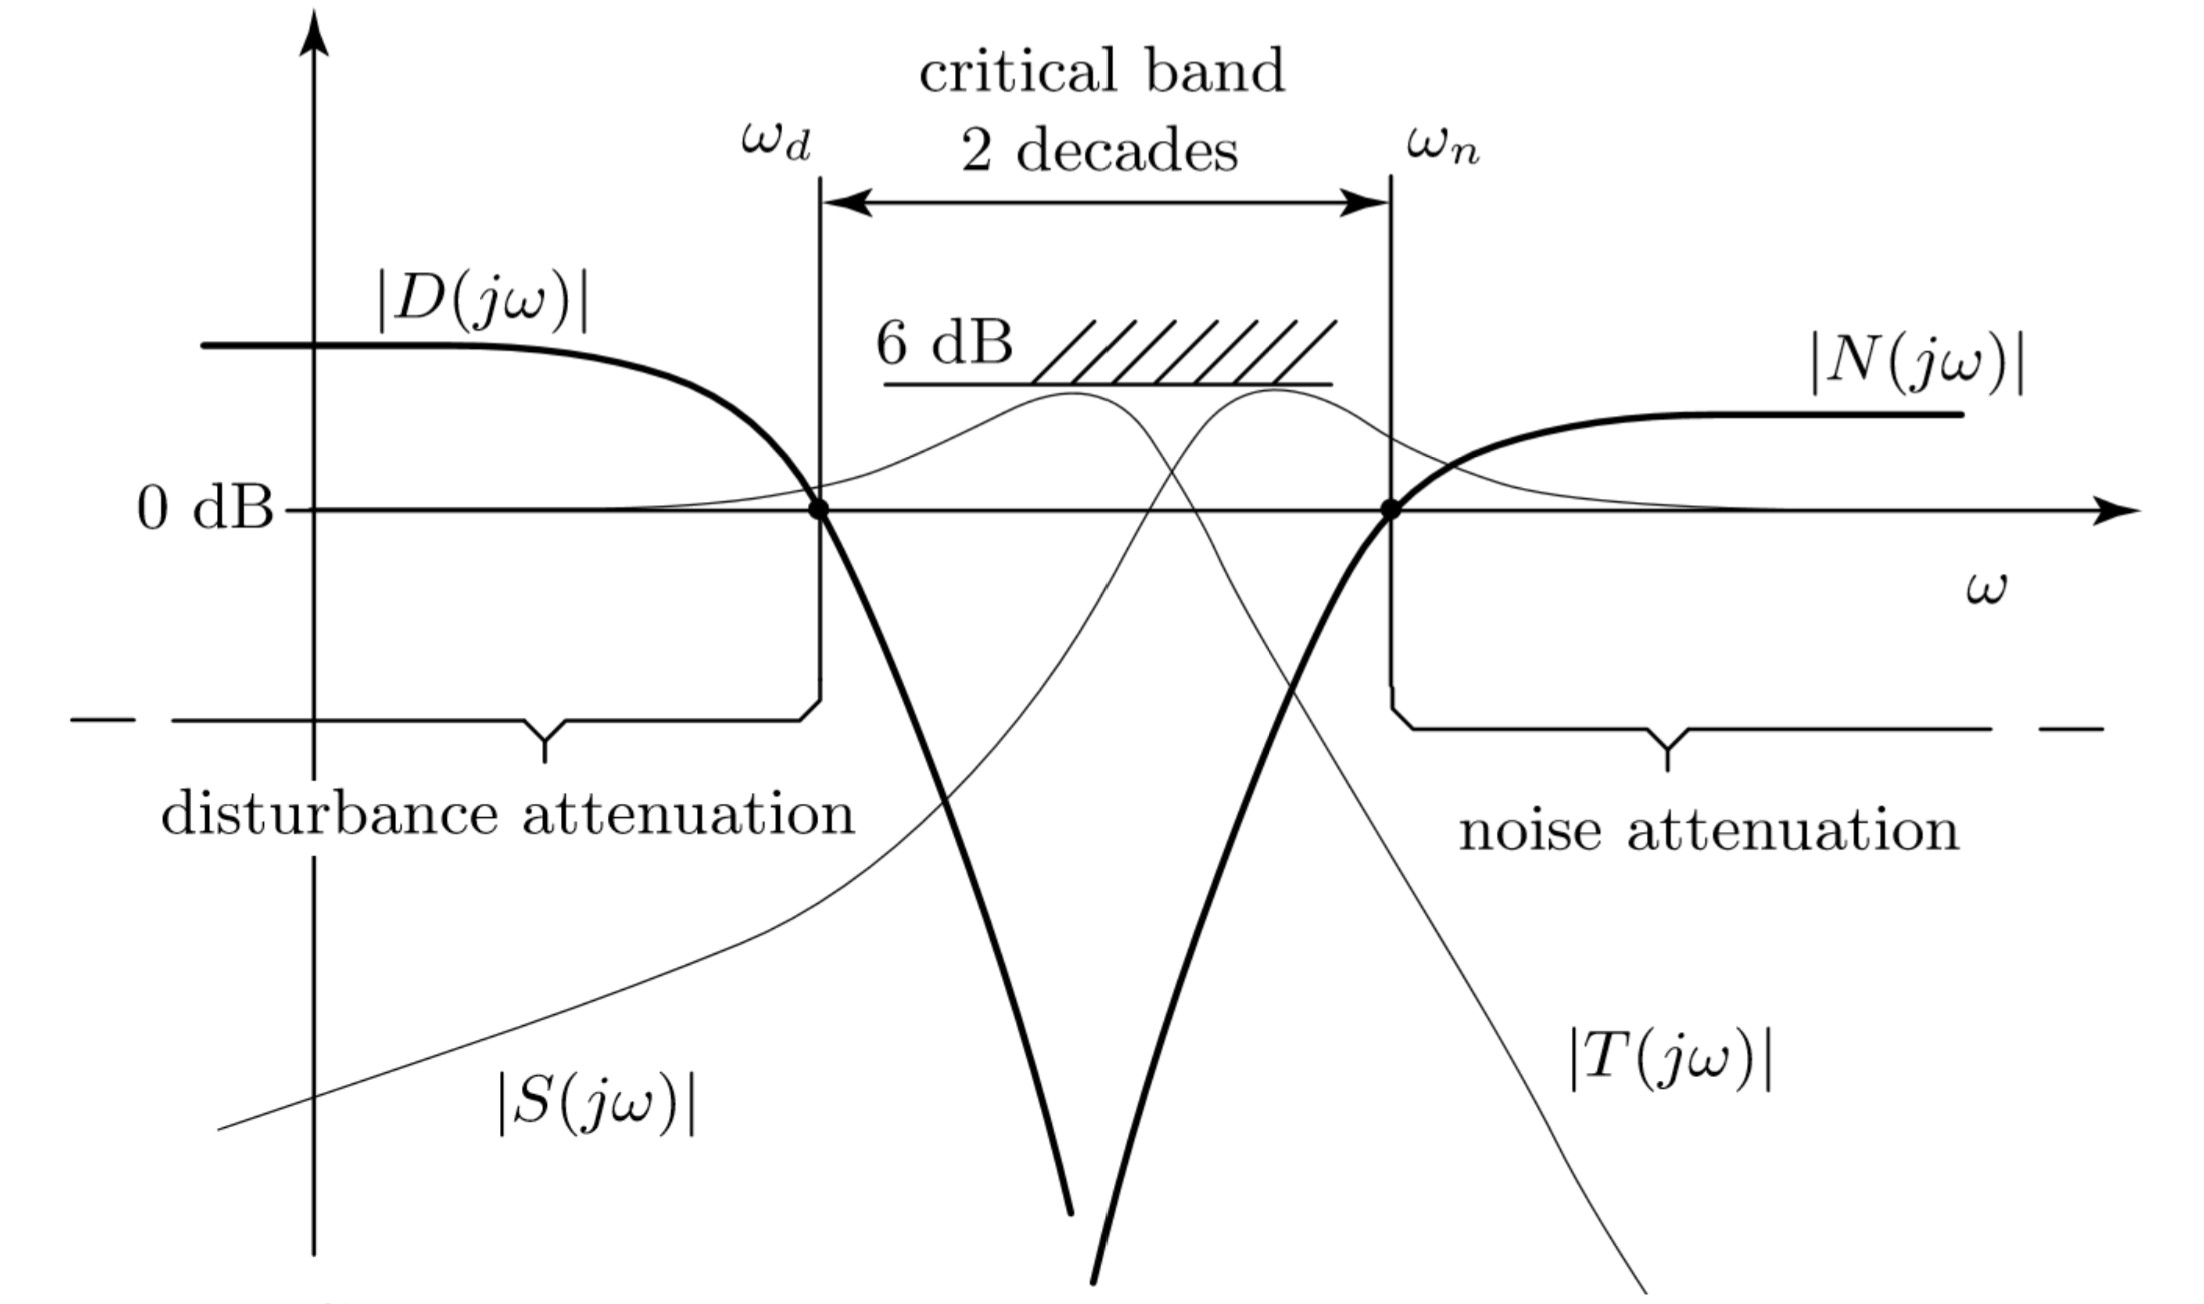
\includegraphics[width = \linewidth]{images/08/Stoerung_und_Rauschen.jpg}
        \subsubsection{Beschränkung der Sensitivität}
            Der Frequenzgang der Sensitivität $S(j\omega)$ kann durch Einstellen des Reglers $C(j\omega)$ lokal beeinflusst werden.
            
            Global betrachtet, über alle $\omega$, muss die Sensitivität für alle stabilen geschlossenen Regelkreise (d.h. Stabilität durch das Nyquist Theorem bestimmt) folgende Gleichung erfüllen:
            \[
            \int_0^\infty ln|S(j\omega)|d\omega = \pi \cdot \sum^{n_+}_{i=1} \pi^+_i
            \]
            
            wobei $n^+$ die Anzahl der instabilen Pole $\pi^+$ der Kreisverstärkung $L(s)$ ist. Diese Gleichung impliziert dass eine Verringerung von $|S(j\omega)|$ in einem Frequenzband durch eine Erhöhung in einem anderen Frequenzband kompensiert wird. Falls die Kreisverstärkung $L(s)$ keine instabilen Pole ($n_+=0$) vereinfacht sich die Gleichung zu:
            \[\int_0^\infty ln|S(j\omega)|d\omega = 0\]
    \subsection{Beschränkung der Durchtrittsfrequenz}
    
        $\omega_c$ ist die \textbf{Durchtrittsfrequenz}, und entspricht der Frequenz bei der das Bode-Diagramm von $L(j\omega)$ die 0dB-Linie schneidet\\
        $\omega_b$ ist die \textbf{Bandbreite} des geschlossenen Regelkreises. Die Bandbreite ist ein Mass für die höchste Frequenz des Eingangssignals, die der geschlossene Regelkreis verfolgen kann.
        
        Beim \textbf{geschlossenen Regelkreis:} $\omega_b:=|T(j\omega_b)|=-3dB\approx 0.7$\\
        Die Bandbreite entspricht ungefähr der Durchtrittsfrequenz. $\boxed{\omega_b\approx\omega_c}$

        Zusammenfassend kann man folgende Formel für die Beschränkung Anwenden:
        
        \[\boxed{\omega_c = 
        \begin{cases}
        \omega_c > \textrm{max}\{10\cdot\omega_d, 2\cdot\omega_{\pi^+}\}\\
        \omega_c < \textrm{min}\{\frac{1}{10}\cdot\omega_n, \frac{1}{10}\cdot \omega_2, \frac{1}{2}\cdot \omega_\tau, \frac{1}{2}\cdot \omega_{\zeta^+}\}
        \end{cases}
        }
        \]
        
        \subsubsection{Beschränkung durch Modellunsicherheiten $W_2$}
            aus dem robusten Stabilitätskriterium folgt: 
            \[|L(j\omega)\cdot W_2(j_\omega)| < |1+L(j\omega)|, \forall \omega\in[0,\infty)\]
            \[\Rightarrow \bigg|\frac{L(j\omega)}{1+L(j\omega)}\bigg|<\bigg|\frac{1}{W_2(j\omega)}\bigg|\]
            \[\Rightarrow |T(j\omega)|<\big|W_2^{-1}(j\omega)\big|\]
            Da die Unsicherheit $|W_2(j\omega)|$  tendenziell mit der Frequenz zunimmt
            ergibt sich dadurch eine \textbf{obere} Grenze der Bandbreite, und somit eine Beschränkung der Durchtrittsfrequenz von $|L(j\omega)|$.
            
            Man will die Unsicherheit auf jeden Fall vermeiden. Deswegen wählt man als obere Schranke für die Durchtrittsfrequenz eine Dekade kleiner als die Unsicherheitsfrequenz.
            \[\boxed{\omega_c\overset{!}{<}\mathbf{\frac{1}{10}}\cdot\omega_2} \hspace{5mm}|W_2(j\omega_2)|=1\]
        \subsubsection{Beschränkung durch eine Totzeit $\tau$}
            Die Übertragungsfunktion der Kreisverstärkung mit Verzögerung im Regler und der Regelstrecke ist gegeben durch: 
            \[L_\tau(s) = C(s)\cdot P(s)\cdot e^{-(\tau C + \tau P)\cdot s} = C(s) \cdot P(s) \cdot e^{-\tau\cdot s}\]
                
            Die Totzeit induziert eine \textbf{obere} Grenze für die Durchtrittsfrequenz. Um die Totzeitsfrequenz gut zu vermeiden wird als Grenze die halbe Totzeitfrequenz gewählt.
            \[\boxed{\omega_c \overset{!}{<}\mathbf{\frac{1}{2}} \cdot \omega_\tau = \frac{1}{2}\cdot\frac{1}{\tau}}\hspace{5mm} (\textrm{konservativer mit } \mathbf{\frac{1}{5}} \textrm{ als Faktor)}\]
        \subsubsection{ Beschränkung durch nicht-minimalphasige Nullstellen $\omega_{\zeta^+}$}
        Gegeben sei eine Regelstrecke $P(s) = \frac{n(s)}{d(s)}$ mit mindestens einer nicht-minimalphasigen Nullstelle. Um die Wirkung der Nullstellen zu veranschaulichen, wählt man einen konstanten Regler $C(s) = k_p$, $k_p \in \mathbb{R}$.
        \[S(s) = \frac{d(s)}{d(s)+k_p\cdot n(s)}, \hspace{5mm} T(s) = \frac{k_p\cdot n(s)}{d(s)+k_p\cdot n(s)}\] 
        
        Wenn $k_p \rightarrow \infty$ strebt, nähern sich die Pole von $S(s)$ und $T(s)$, gegeben durch $d(s)+k_p \cdot n(s) = 0 $, an die Lösung von $n(s) = 0$. Da $n(s)$ mindestens eine nicht-minimalphasige Nullstele hat, wird das System bei $k_p = k_{p,\textrm{crit}}$ instabil. Dies impliziert, dass die Bandbreite durch eine \textbf{obere} Grenze beschränkt ist.
        \[\boxed{\omega_c \overset{!}{<} \mathbf{\frac{1}{2}} \cdot\omega_{\zeta^+}} \hspace{5mm} (\textrm{konservativer mit } \mathbf{\frac{1}{5}}\textrm{ als Faktor})\]
        
        \subsubsection{Beschränkung durch instabile Pole $\pi^+$}
            \begin{itemize}
                \item \textbf{Instabile Pole $\mathbf{\pi^+}$ ohne Modellierungsunsicherheit}

                Nominelles Stabilitätskriterium von Nyquist prüfen der Regler so auslegen, dass das Kriterium für die Kreisverstärkung $L(S)$ erfüllt ist
                
                Daraus folgt eine \textbf{untere} Schranke für die Durchtrittsfrequenz:
                
                \[\boxed{\omega_c>\mathbf{2}\cdot \omega_{\pi^+}}\hspace{5mm} (\textrm{konservativer mit } \mathbf{5}\textrm{ als Faktor})\]
                
                \item \textbf{Instabile Pole $\mathbf{\pi^+}$ mit Modellierungsunsicherheit}\\
                zusätzlich zum Vorhergehenden Vorgehen müssen wir für instabile Pole mit Modellierungsunsicherheit zusätzlich noch \[|W_2(\pi_i^+)| <1, \forall i\]
            \end{itemize}
            
    \subsection{Statischer Nachlauffehler}
        Einfluss des Fehlers $e(t)$ im eingeschwungenen Zustand. Dazu wird der Regelkreis im Frequenzbereich betrachtet:
        \begin{center}
            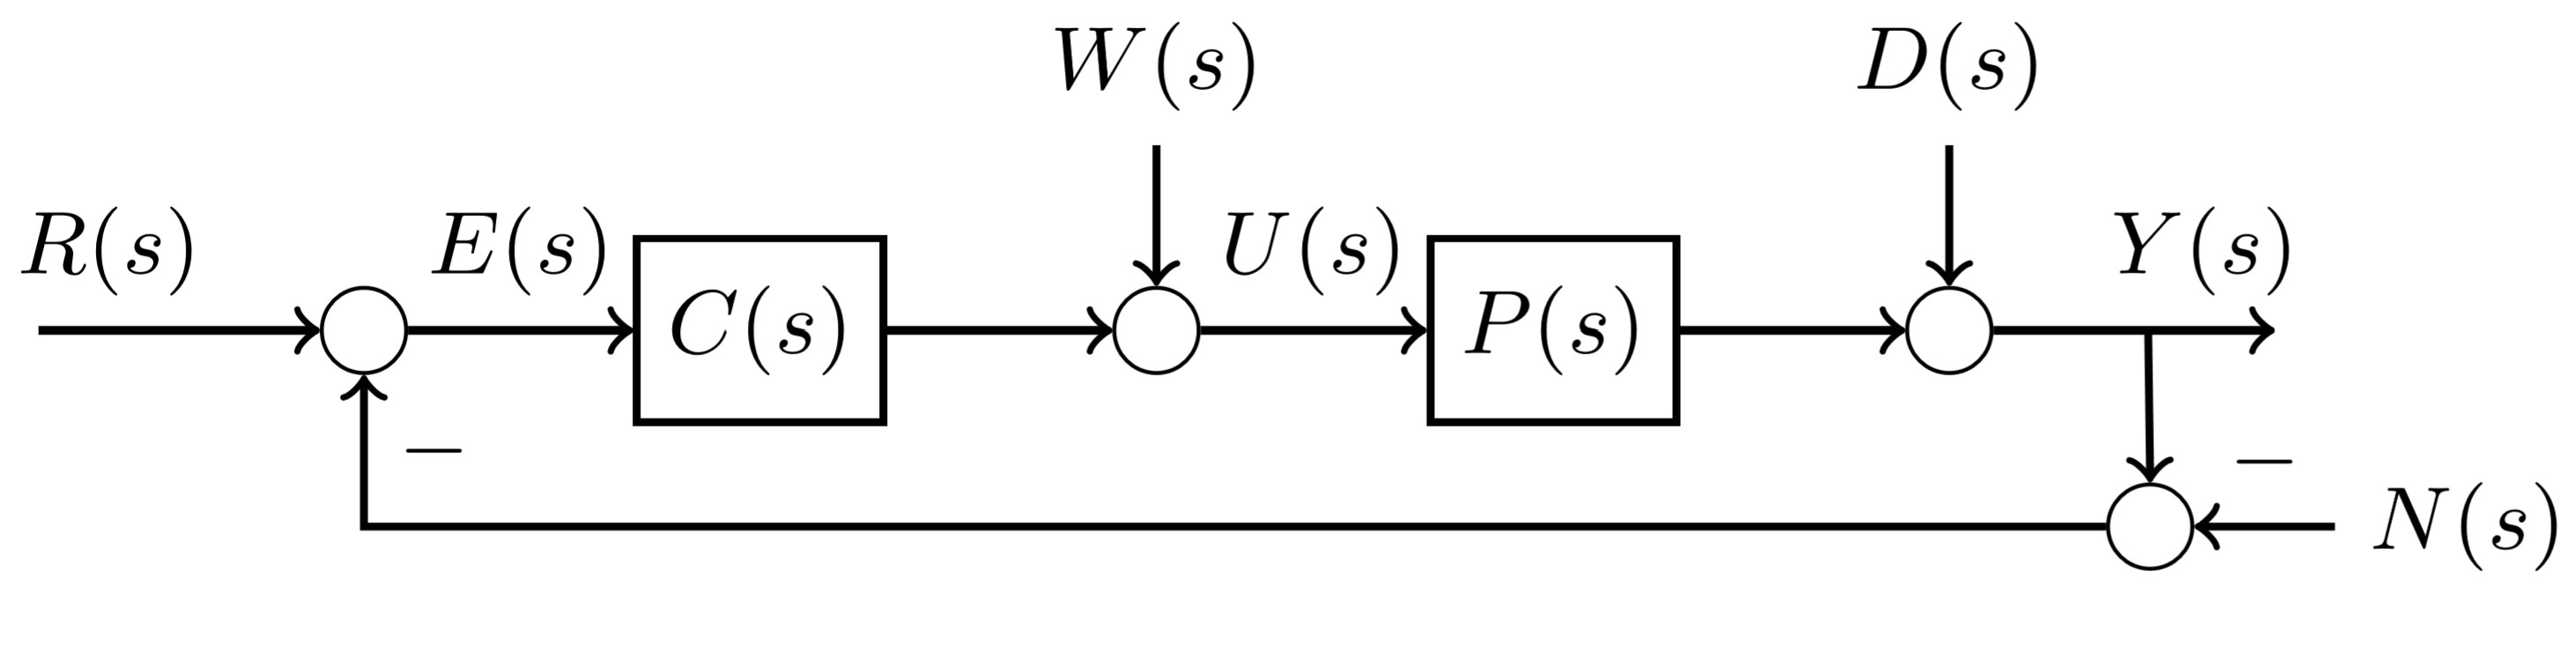
\includegraphics[width = 0.8\linewidth]{images/08/Standart_Regelkreis_FB.jpg}
        \end{center}
        $E(s)$ als Funktion der Eingänge beschrieben: 
    
        \begin{align*}
            E(s) &= E_R(S) + E_N(S) + E_D(s) + E_W(S)\\
            &= \mathbf{S(s)\cdot \left[R(s) + N(s) - D(s) - P(s)\cdot W(s)\right]}
        \end{align*}
        
        Falls der Eingang ($R(s),N(s),-D(s)$) ein Step ist, kann man den Fehler aus dem Endwerttheorem berechnen durch:
        \[e^h_\infty=\lim_{s\to 0_+}s\cdot S(s)\cdot\frac{1}{s}=\lim_{s\to 0_+}S(s)=S(0)\]
        
        \textbf{Achtung:} Aufpassen bei $D(s)$ \& $W(s)$! Bei $D(s)$ das - und bei $W(s)$ multiplizieren mit $-P(s)$ nicht vergessen.
        
        \subsubsection{Bsp}
            \[L_1(s) =\frac{1}{s+1}(k=0),\qquad L_2 =\frac{1}{s(s+1)}(k=1)\]
            \[T_1 =\frac{1}{s+2},\qquad T_2 =\frac{1}{s^2+s+1}\]
            Erstes System hat Systemtyp $k=0$ und weist somit einen Fehler in der Sprungantwort auf: $S_1(0)=\frac{1}{2}$.\\
            Der zweite offene Regelkreis $L_2(s)$ hat Systemtyp $k=1$ ($L_2(s)$ strebt für $s\to 0$ linear gegen $\infty$). Daraus folgt, dass das zweite System fehlerfrei zum Sprung konvergiert.
            \begin{center}
                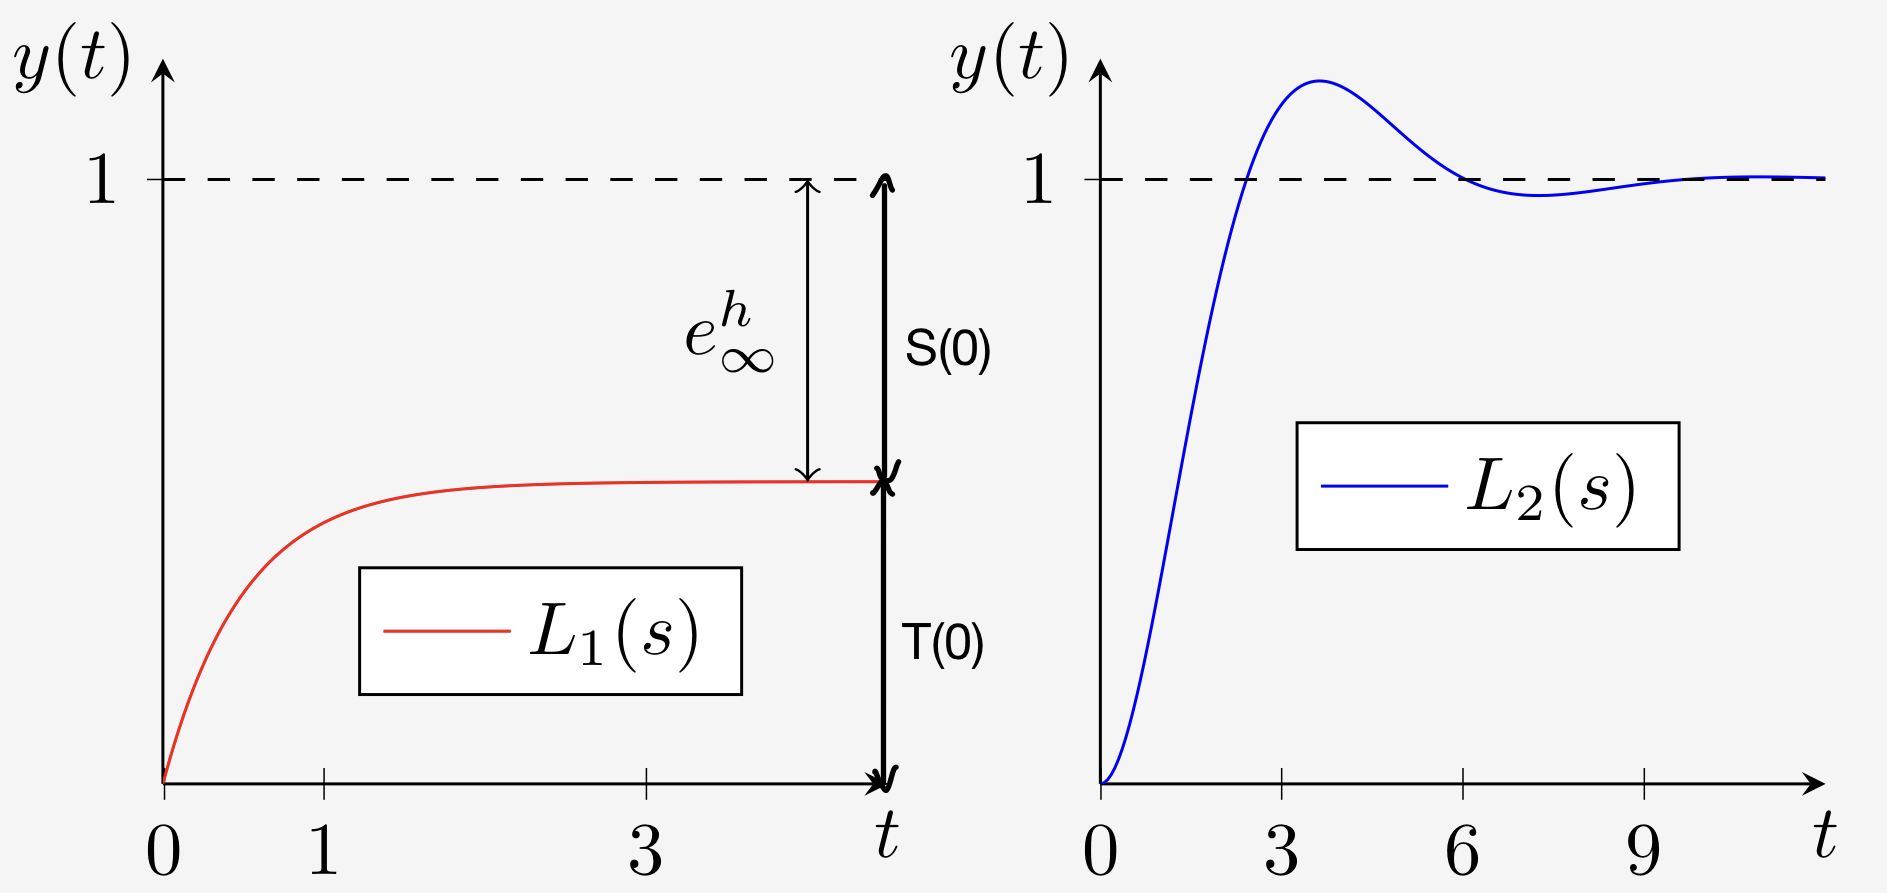
\includegraphics[width=0.8\linewidth]{08/nachlauffehler.jpeg}
            \end{center}

            %$L_1(s)=\frac{1}{s+1}(k=0),\quad L_2=\frac{1}{s(s+1)}(k=1),$
        % man betrachtet Referenzen und Störungen die als Sprünge $h(t)$ auf den Fehler abgebildet werden:
    
        % \[h(t) = 1, \hspace{2mm} t>0 \hspace{3mm} \rightarrow \hspace{3mm} H(s) = \frac{1}{s}\]
    
        % Mit dem Endwerttheorem kann man den Fehler auf eine Sprungantwort nach langer Zeit berechnen: 
        % \TODO{unklar}
    \subsection{Spezifikationen basierend auf   Systeme 2. Ordnung}
        Es wird angenommen, dass der geschlossene Regelkreis $T(S)$ einem System zweiter Ordnung entspricht:
        \[T(s) = \frac{\omega_0^2}{s^2+2\cdot\delta\cdot\omega_0\cdot s+\omega_0^2}\] 
        Dieser Regelkreis $T(s)$ soll Spezifikationen in der Anstiegszeit \textcolor{blue}{$t_{90}$} und im relativen Überschwingen \textcolor{red}{$\hat{\epsilon}$} erfüllen.
        \begin{center}
            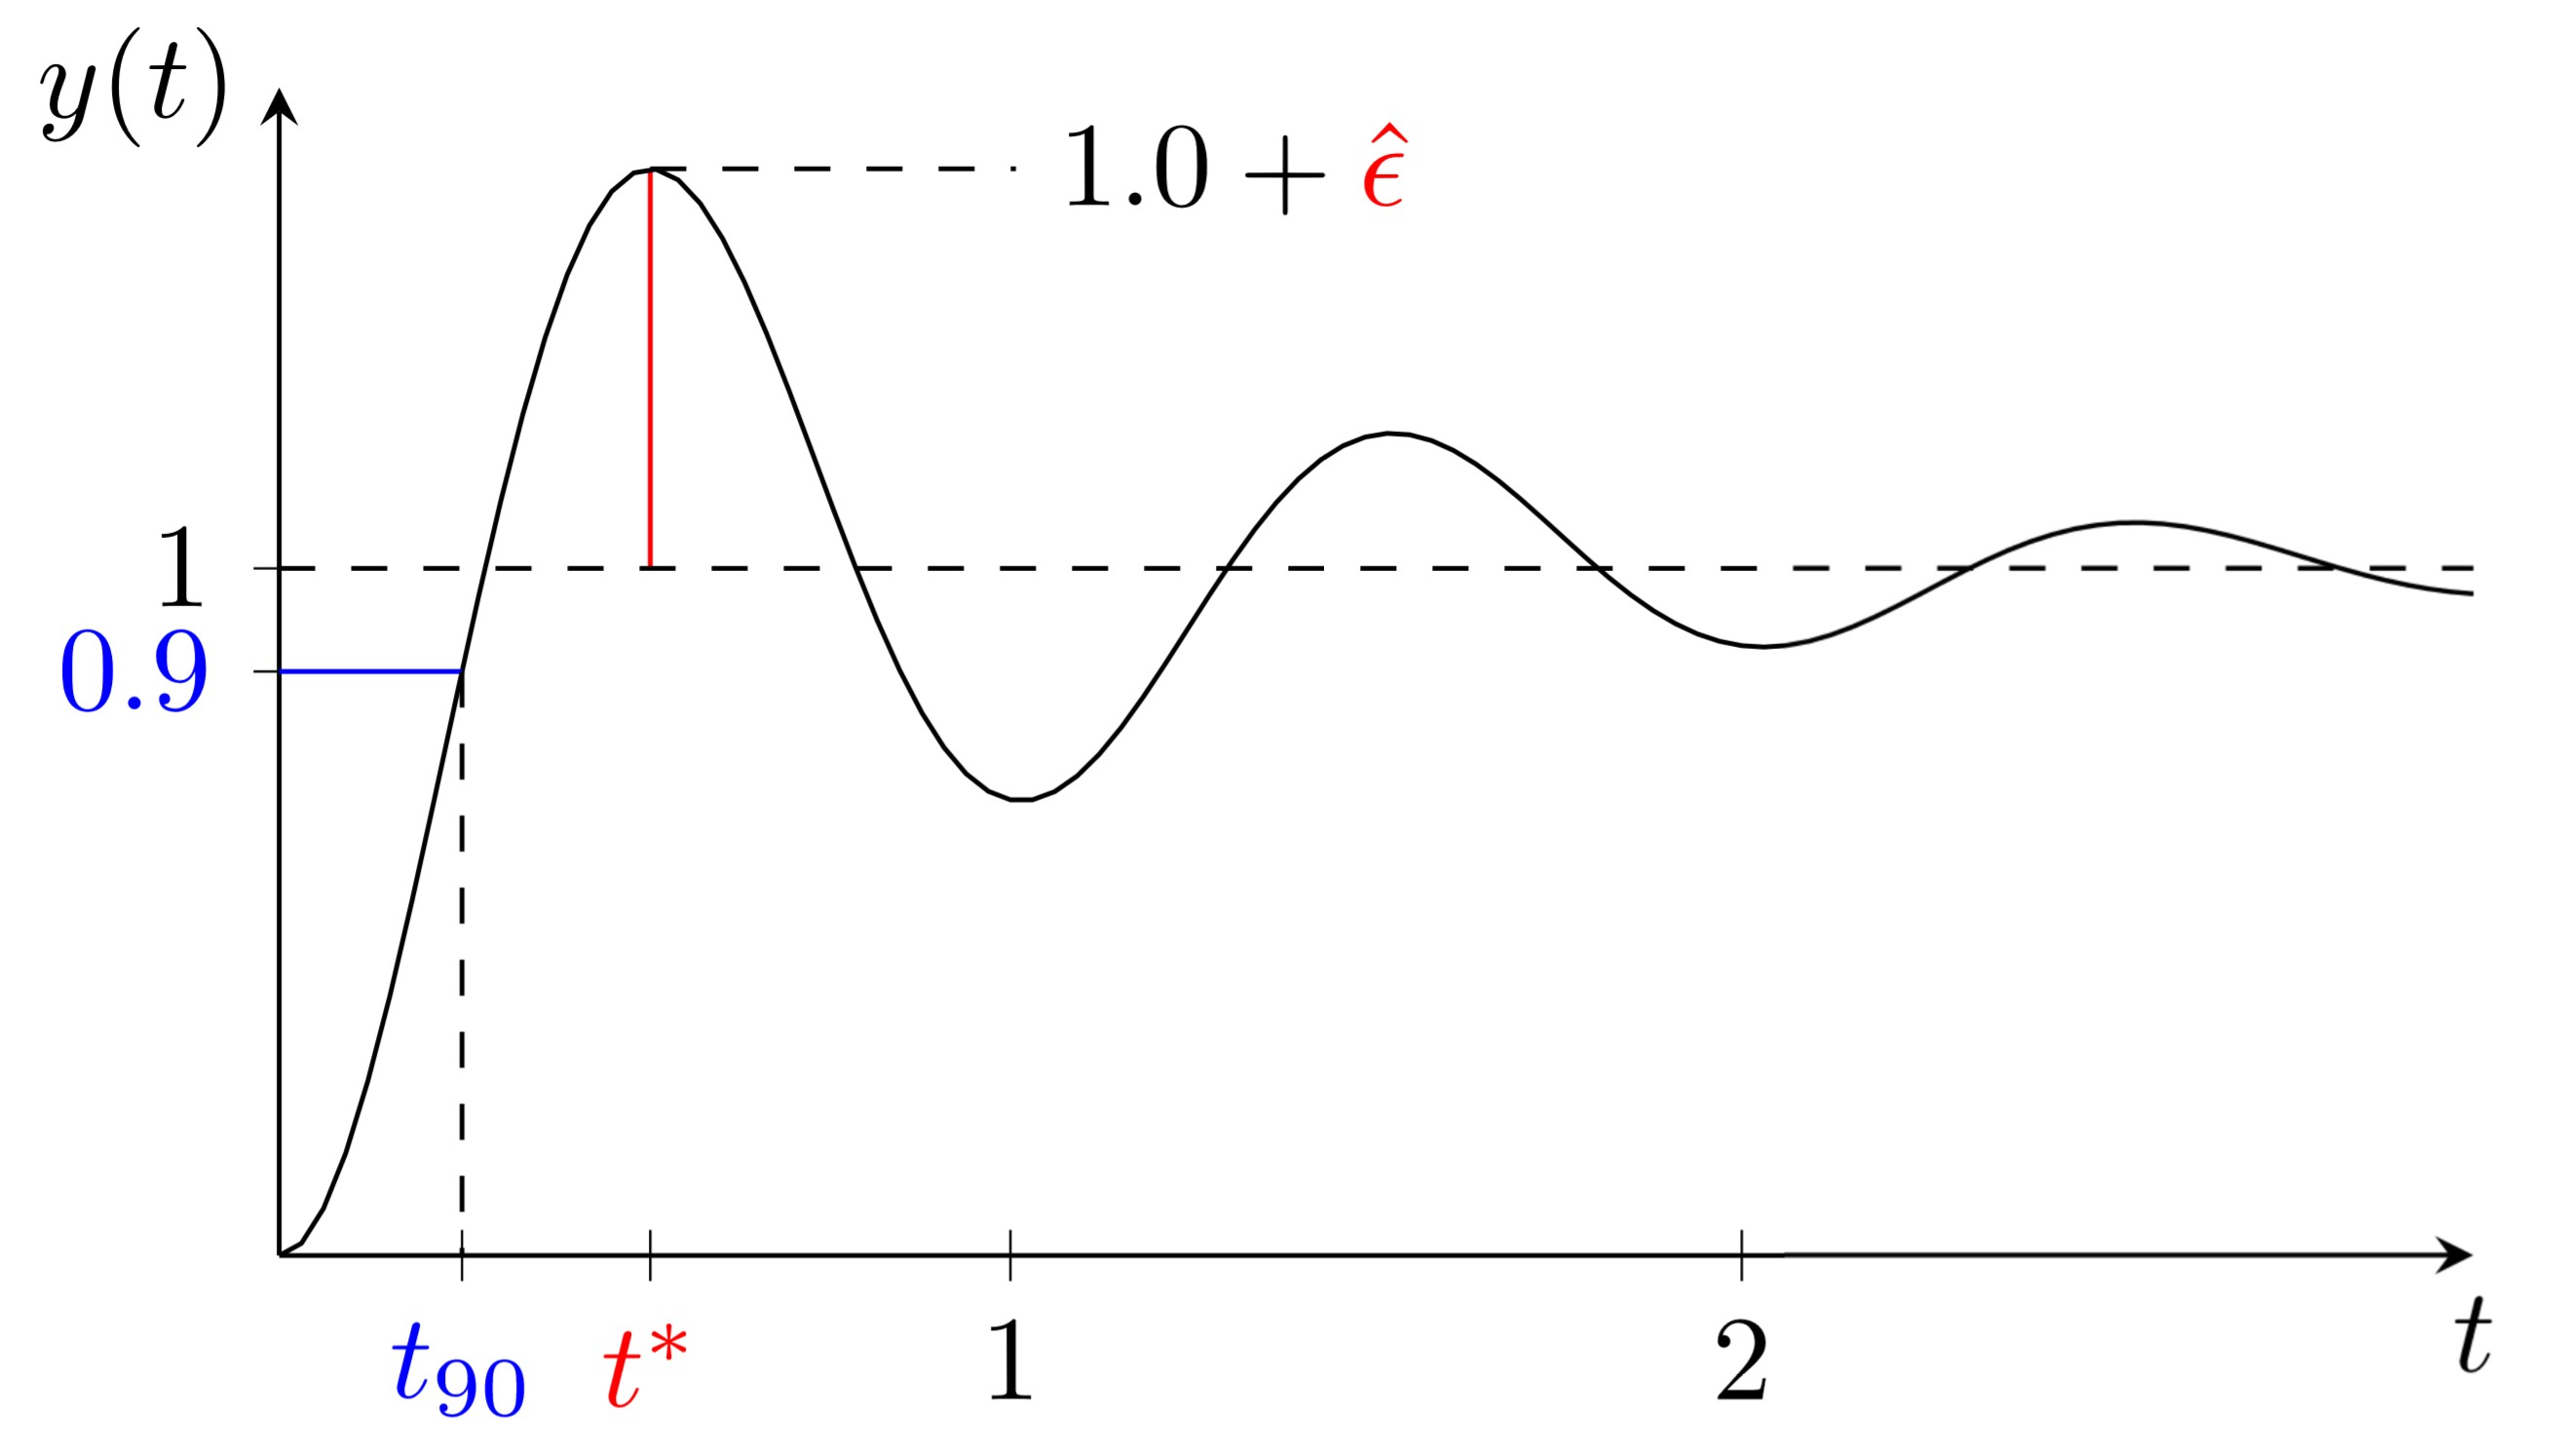
\includegraphics[width = 0.8\linewidth]{images/08/t90_epsilon.jpg}
        \end{center}
    
        gewünschte $\hat{\epsilon}$ und $t_{90}$ können durch auswählen der typischen Parametern eines System 2- Ordnung erreicht werden.
        \[\delta = \frac{-ln(\hat{\epsilon})}{\sqrt{\pi^2+ln^2(\hat{\epsilon})}}, \hspace{3mm} \omega_0 = (0.14 +0.4\cdot\delta)\cdot\frac{2\cdot\pi}{t_{90}} \]
        Nun werden die Spezifikationen an $T(s)$ in Anforderungen an die Kreisverstärkung $L(s)$ umgewandelt, unter Anwendung von $T(s) = \frac{L(s)}{1+L(s)}$.
    
        Die Anforderungen des geschlossenen Regelkreises können in Anforderungen an die Durchtrittsfrequenz $\omega_c$und die Phasenreserve $\varphi$ der Kreisverstärkung $L(s)$ umformuliert werden:
    
        \begin{align*}
            \omega_c &= \omega_0\cdot \sqrt{\sqrt{4\cdot\delta(\hat{\epsilon})^4+1}-2\cdot\delta(\hat{\epsilon})^2}\\
            \varphi &= \frac{\pi}{2}-\arctan\Bigg(\frac{ 
            \sqrt{\sqrt{4\cdot\delta(\hat{\epsilon})^4+1}-2\cdot\delta(\hat{\epsilon})^2}}{2\cdot\delta(\hat{\epsilon})}\Bigg)
        \end{align*}
    
        diese Gleichungen können für $\boxed{0.45<\delta<1}$ mit den folgenden vereinfachten Zusammenhängen angenähert werden:
        \begin{center}
            \begin{tabular}{|l c l|}
                \hline
                &&\\
                $\omega_c$   &  $\approx$ &       $\frac{1.7}{t_{90}}$\\
                &&\\
                $\varphi$   & $\approx$ &         $71^\circ-117^\circ\cdot\hat{\epsilon}    $\\
                &&\\
                \hline
            \end{tabular}
        \end{center}
        (Systeme mit Dämpfungen $\delta$ ausserhalb der Menge $(0.45,1)$ sind in der Praxis nicht relevant, weil sie entweder sehr stark überschwingen oder extrem langsam sind.)
    \subsection{Frequenzbereich - Spezifikationen}
        Die Störung $D(s)$ und das Rauschen $N(s)$ werden durch die Sensitivität $S(s)$ und durch die komplementäre Sensitivität $T(s)$ auf den Ausgang abgebildet:
        \[Y(j\omega) = S(j\omega)\cdot D(j\omega)+T(j\omega)\cdot N(j\omega)\]
        
        Um die Auswirkung von Störungen und Rauschen um die Durchtrittsfrequenz $\omega_c$ zu minimieren, beschränkt man den Maximalwert von $S(s)$ und $T(s)$.
        
        \[
        \|S\|_\infty<S_{max}, \hspace{3mm} \|T\|_\infty < T_{max}, \hspace{3mm} S_{max},T_{max} > 1,
        \]
        wobei per Definition $\|\Sigma\|_\infty = max_\omega|\Sigma(j\omega)|$.
        
        Diese Bedingungen werden in Anforderungen an die Kreisverstärkung $L(s)$ umgewandelt:
        
        \begin{align*}
            \|S\|_\infty &< S_{max} \Leftrightarrow L(j\omega) \notin \Bigg\{|1+z|\leq \frac{1}{S_{max}}\Bigg| z\in\mathbb{C}\Bigg\}\\
            \|T\|_{\infty} &< T_{max} \Leftrightarrow L(j\omega)\notin\Bigg\{\Bigg|\frac{T_{max}^2}{T_{max}^2-1}+z\Bigg| \leq \frac{T_{max}}{T^2_{max}-1}\Bigg|z\in\mathbb{C}\Bigg\}
        \end{align*}
%\vfill\null\columnbreak        
        \subsubsection{geometrische Interpretation}
           \textbf{Die geometrische Interpretation von} 
            \[L(j\omega) \notin \Bigg\{|1+z|\leq \frac{1}{S_{max}}\Bigg| z\in\mathbb{C}\Bigg\}\]
            \begin{center}
                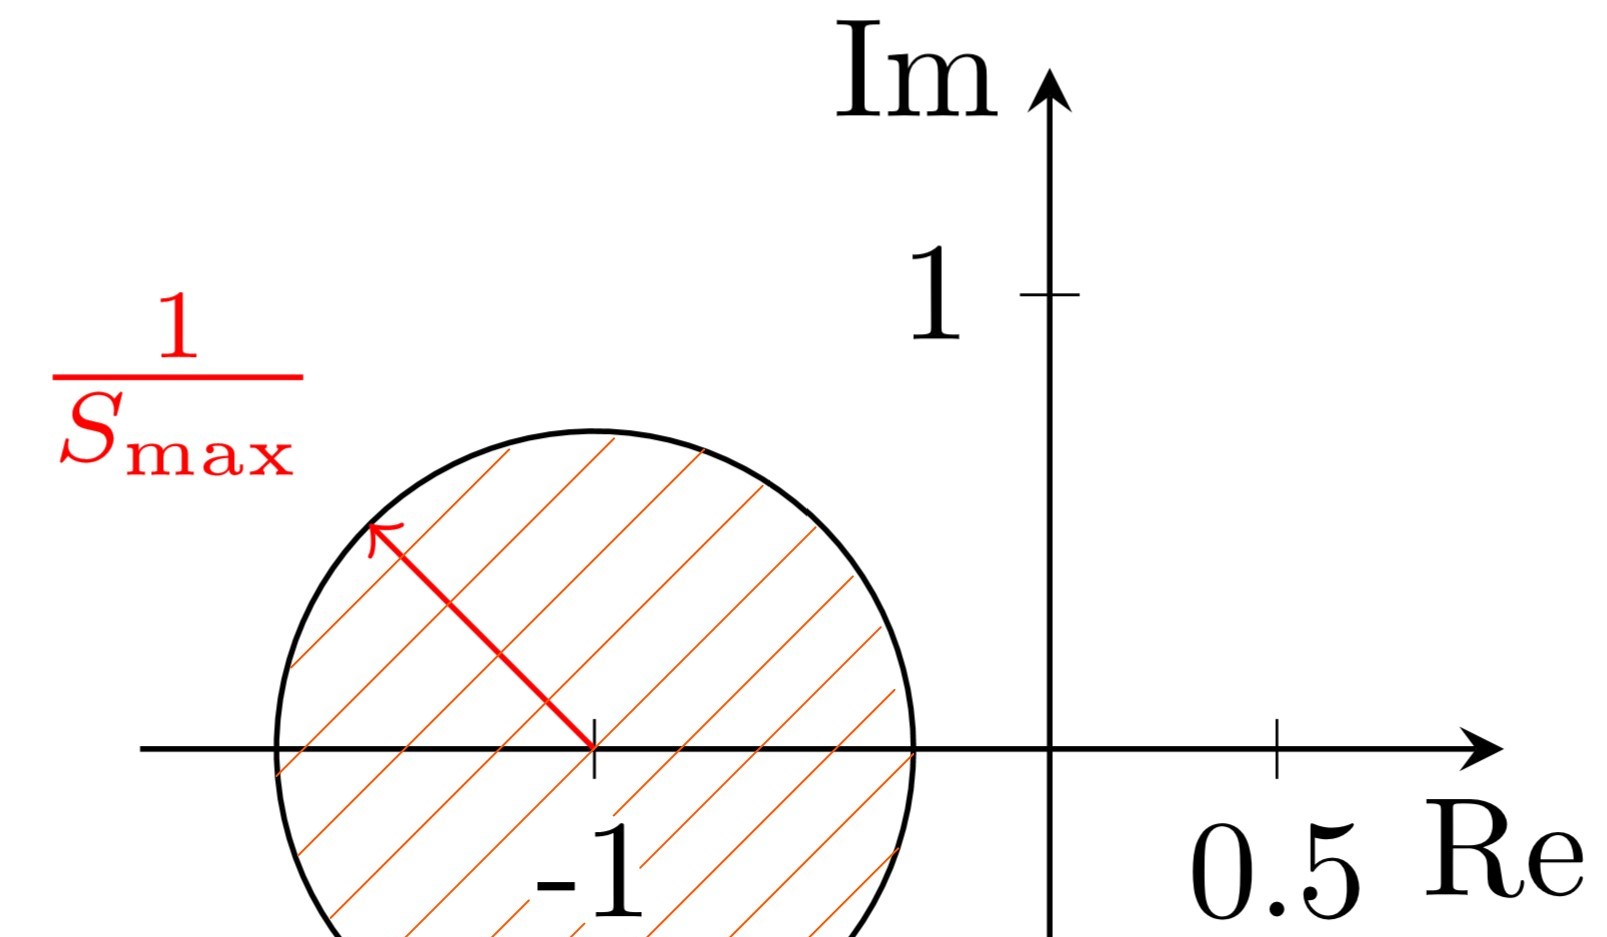
\includegraphics[width = 0.6\linewidth]{images/08/Spezifikation_im_FB.jpg}
            \end{center}
         $L(j\omega)$ darf nicht in einem in -1 zentrierten Kreis mit Radius $\frac{1}{S_{max}}$ eintreten.
         
            \textbf{Die geometrische Interpretation von}
            \[L(j\omega)\notin\Bigg\{\Bigg|\frac{T_{max}^2}{T_{max}^2-1}+z\Bigg| \leq \frac{T_{max}}{T^2_{max}-1}\Bigg|z\in\mathbb{C}\Bigg\}\]
            \begin{center}
                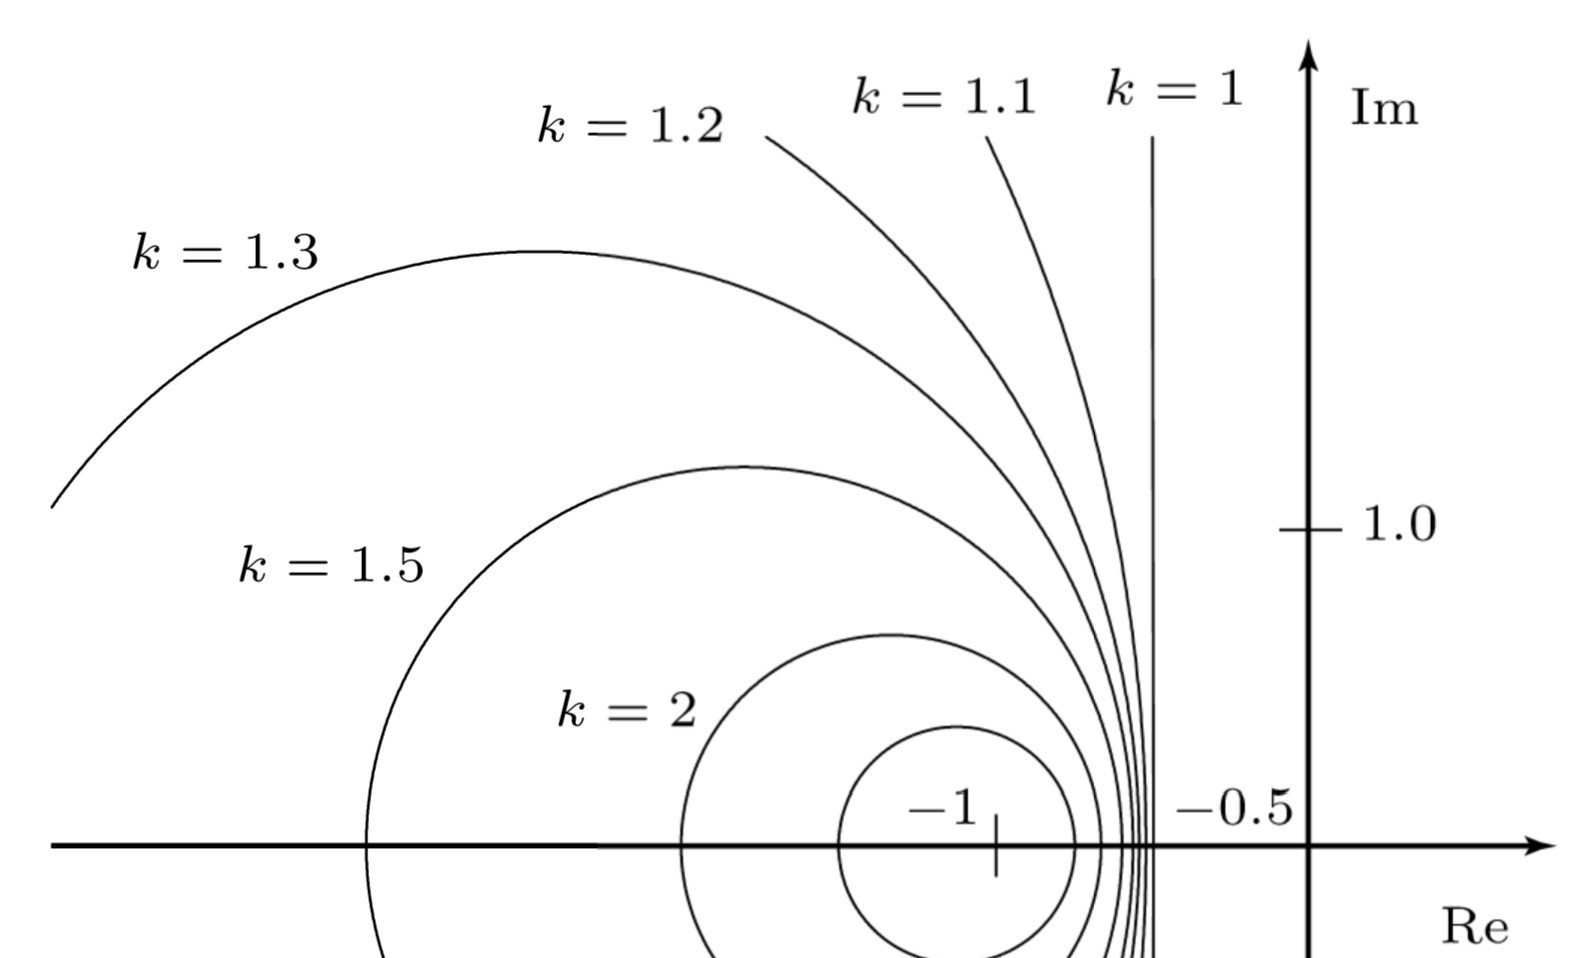
\includegraphics[width = 0.8\linewidth]{images/08/Spezifikation_im_FB2.jpg}
            \end{center}
            $L(j\omega)$ darf nicht in einem in $\frac{-T^2_{max}}{T^2_{max}-1}$ zentrierten Kreis mit Radius $\frac{T_{max}}{T^2_{max}-1}$ eintreten.
